\chapter{Results}\label{chapter:Results}
Present the results from following the procedures in \nameref{chapter:Method}, note some observations, but do not discuss them.

\begin{table}[h]
    \centering
    \begin{tabular}{l | l | l}
    A & B & C \\
    \hline
    1 & 2 & 3 \\
    4 & 5 & 6
    \end{tabular}
    \caption{very basic table}
    \label{tab:abc}
    \end{table}

\section{Simulations with 'cheap FSI'}
As there are many simulations in total, not all will be shown. Rather, a few simulations will be selected as representatives in order to study the effect that different slit defects, element sizes, materials and pressure amplitudes has on the response of the plate.

To study the effect of different slit defect geometries, the final deformation mode of four select simulations, corresponding to the four plates in Figure \ref{fig:plates}, are shown in Figure \ref{fig:effect_slit}. As can be seen in all of them, the slits create "flaps" that open in a petal mode in response to the applied pressure load. At the outer ends of the slits, cracks develop that propagate along the direction of the slits towards the boundary, tearing up the plate. For the plate 4-HV in \ref{fig:4-HV_1p5_T6_15}, cracks from different slits converges and eventually cuts out the centre part, which is then ejected.

\begin{figure}
    \centering
    \begin{subfigure}[b]{0.45\textwidth}
        \centering
        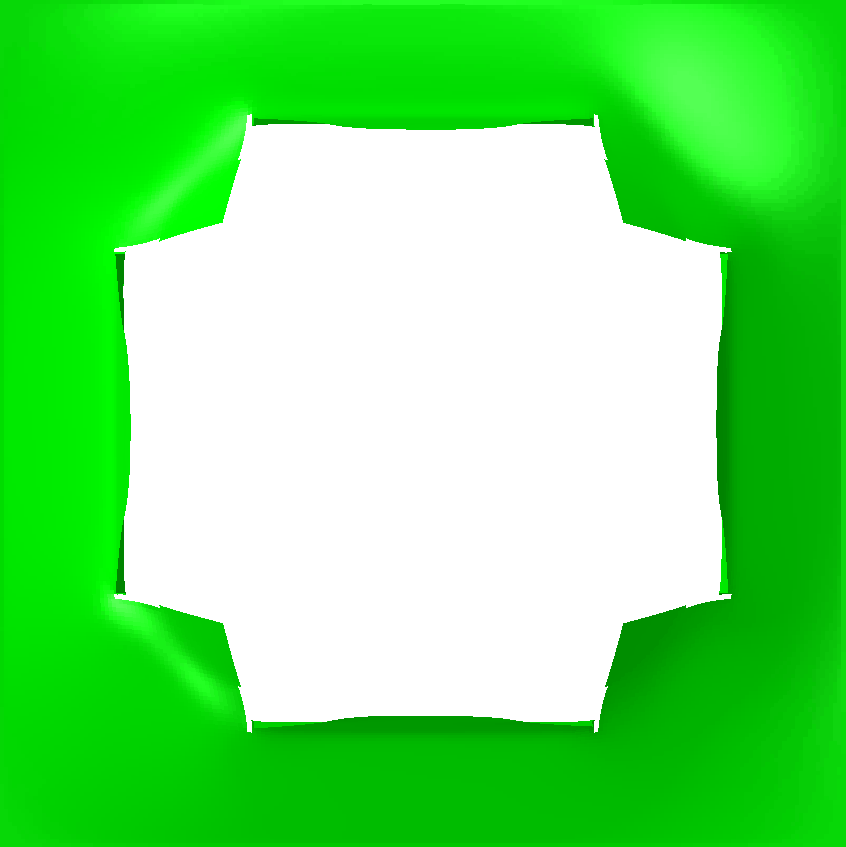
\includegraphics[width=\textwidth]{results/4-HV_1p5_T6_15}
        \caption{\textcolor{tab:red}{\underline{4-HV}}\_1p5\_T6\_15}
        \label{fig:4-HV_1p5_T6_15}
    \end{subfigure}
    \begin{subfigure}[b]{0.45\textwidth}
        \centering
        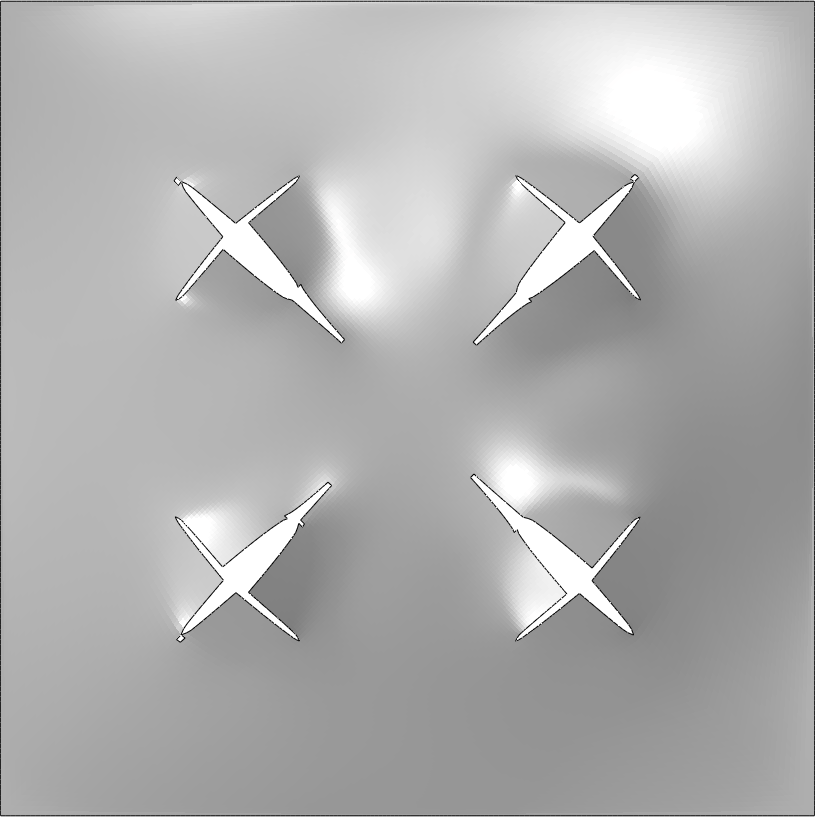
\includegraphics[width=\textwidth]{results/4-45_1p5_T6_15}
        \caption{\textcolor{tab:red}{\underline{4-45}}\_1p5\_T6\_15}
        \label{fig:4-45_1p5_T6_15}
    \end{subfigure}
    \begin{subfigure}[b]{0.45\textwidth}
        \centering
        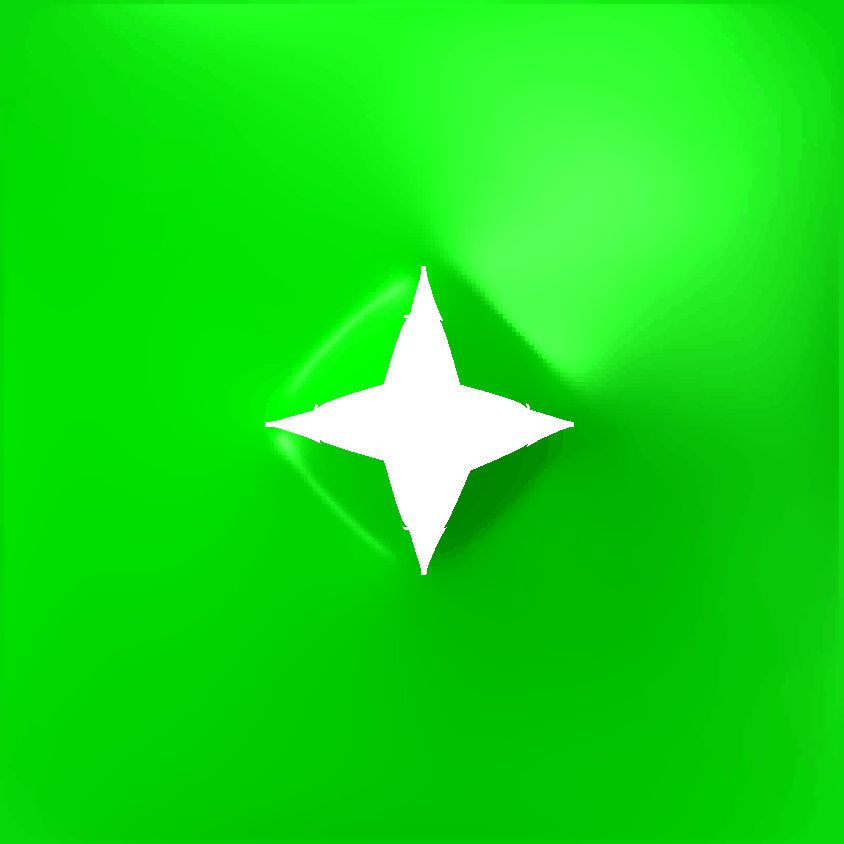
\includegraphics[width=\textwidth]{results/1-HV_1p5_T6_15}
        \caption{\textcolor{tab:red}{\underline{1-HV}}\_1p5\_T6\_15}
        \label{fig:1-HV_1p5_T6_15}
    \end{subfigure}
    \begin{subfigure}[b]{0.45\textwidth}
        \centering
        
\includegraphics[width=\textwidth]{results/1-22p5_1p5_T6_15}
        \caption{\textcolor{tab:red}{\underline{1-22p5}}\_1p5\_T6\_15}
        \label{fig:1-22p5_1p5_T6_15}
    \end{subfigure}
    \caption{Effect of the slits.}
    \label{fig:effect_slit}
\end{figure}

\begin{figure}
    \centering
    \begin{subfigure}[b]{0.45\textwidth}
        \centering
        
\includegraphics[width=\textwidth]{results/1-HV_3p0_T6_15}
        \caption{1-HV\_\textcolor{tab:red}{\underline{3p0}}\_T6\_15}
        \label{fig:1-HV_3p0_T6_15}
    \end{subfigure}
    \begin{subfigure}[b]{0.45\textwidth}
        \centering
        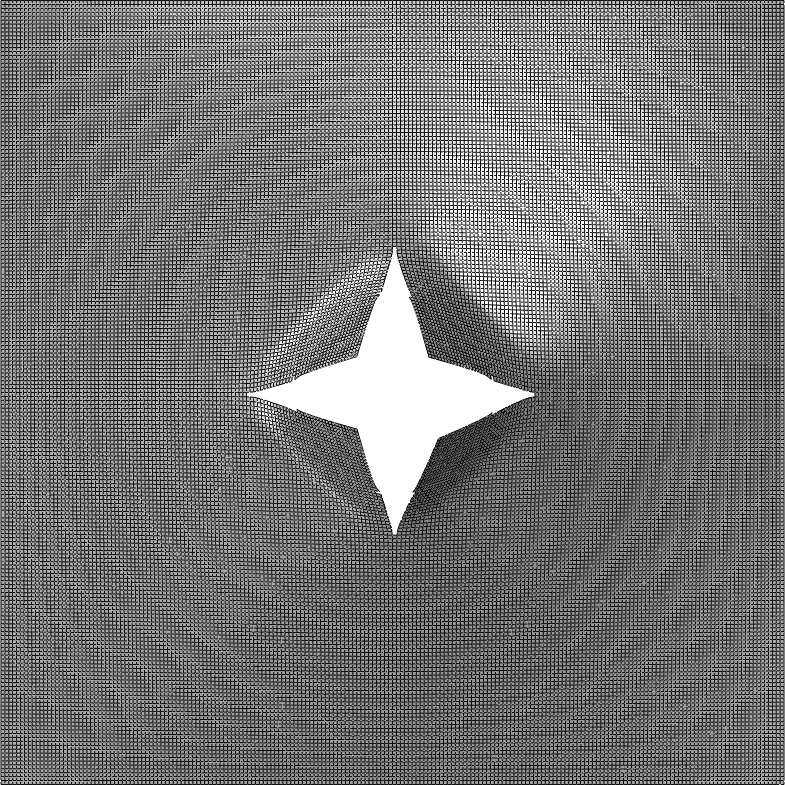
\includegraphics[width=\textwidth]{results/1-HV_1p5_T6_15_mesh}
        \caption{\text{1-HV\_\textcolor{tab:red}{\underline{1p5}}\_T6\_15}}
        \label{fig:1-HV_1p5_T6_15_mesh}
    \end{subfigure}
    \caption{Effect of different element sizes.}
    \label{fig:effect_element}
\end{figure}

\begin{figure}
    \centering
    \begin{subfigure}[b]{0.32\textwidth}
        \centering
        
\includegraphics[width=\textwidth]{results/1-22p5_1p5_T4_15}
        \caption{\text{1-22p5\_1p5\_\textcolor{tab:red}{\underline{T4}}\_15}}
        \label{fig:T4}
    \end{subfigure}
    \begin{subfigure}[b]{0.32\textwidth}
        \centering
        
\includegraphics[width=\textwidth]{results/1-22p5_1p5_T6_15}
        \caption{\text{1-22p5\_1p5\_\textcolor{tab:red}{\underline{T6}}\_15}}
        \label{fig:T6}
    \end{subfigure}
    \begin{subfigure}[b]{0.32\textwidth}
        \centering
        
\includegraphics[width=\textwidth]{results/1-22p5_1p5_T7_15}
        \caption{\text{1-22p5\_1p5\_\textcolor{tab:red}{\underline{T7}}\_15}}
        \label{fig:T7}
    \end{subfigure}
    \caption{Effect of the materials.}
    \label{fig:effect_material}
\end{figure}

\begin{figure}
    \centering
    \begin{subfigure}[b]{0.45\textwidth}
        \centering
        
\includegraphics[width=\textwidth]{results/1-HV_1p5_T6_10}
        \caption{1-HV\_1p5\_T6\_\textcolor{tab:red}{\underline{10}}}
        \label{fig:1-HV_1p5_T6_10}
    \end{subfigure}
    \begin{subfigure}[b]{0.45\textwidth}
        \centering
        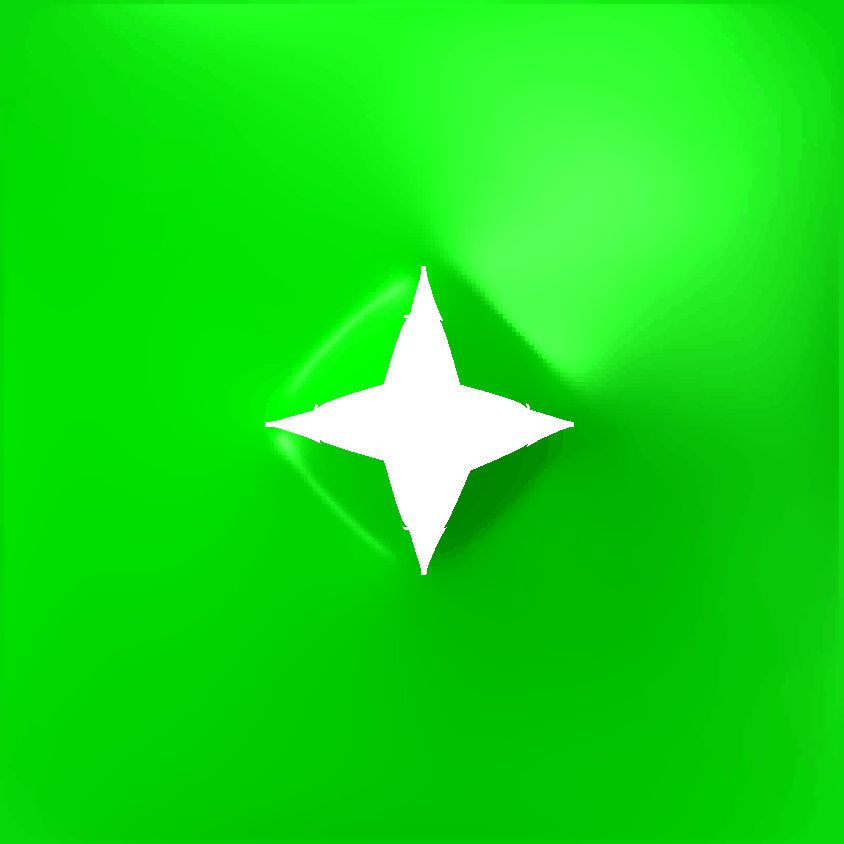
\includegraphics[width=\textwidth]{results/1-HV_1p5_T6_15}
        \caption{1-HV\_1p5\_T6\_\textcolor{tab:red}{\underline{15}}}
        \label{fig:1-HV_1p5_T6_15_amp}
    \end{subfigure}
    \caption{Effect of different pressure amplitudes.}
    \label{fig:effect_amp}
\end{figure}

\section{ANN study with 'cheap FSI'}

\begin{figure}
    \centering
    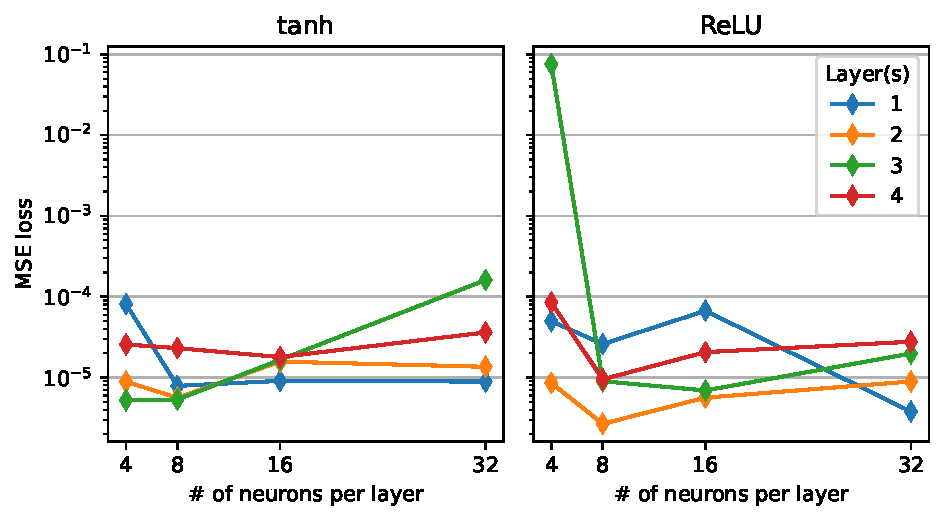
\includegraphics[width=\textwidth]{results/para1_net}
    \caption{Final training losses for different network architectures defined by activation function, number of hidden layers and number of neurons per hidden layer.}
    \label{fig:para1_net}
\end{figure}

\begin{figure}
    \centering
    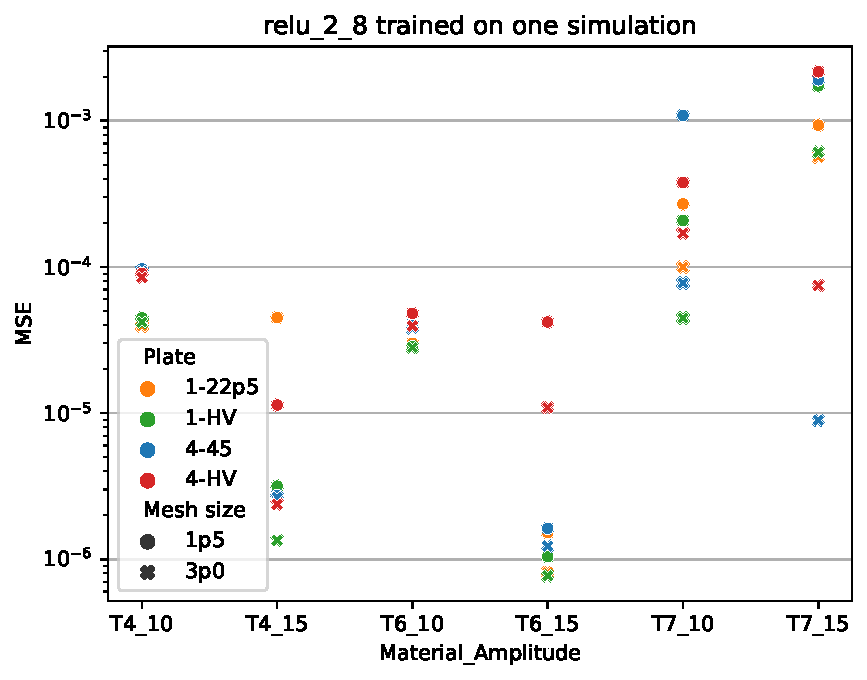
\includegraphics[width=\textwidth]{results/para1_all}
    \caption{Bottom text}
    \label{fig:para1_all}
\end{figure}

\begin{figure}
    \centering
    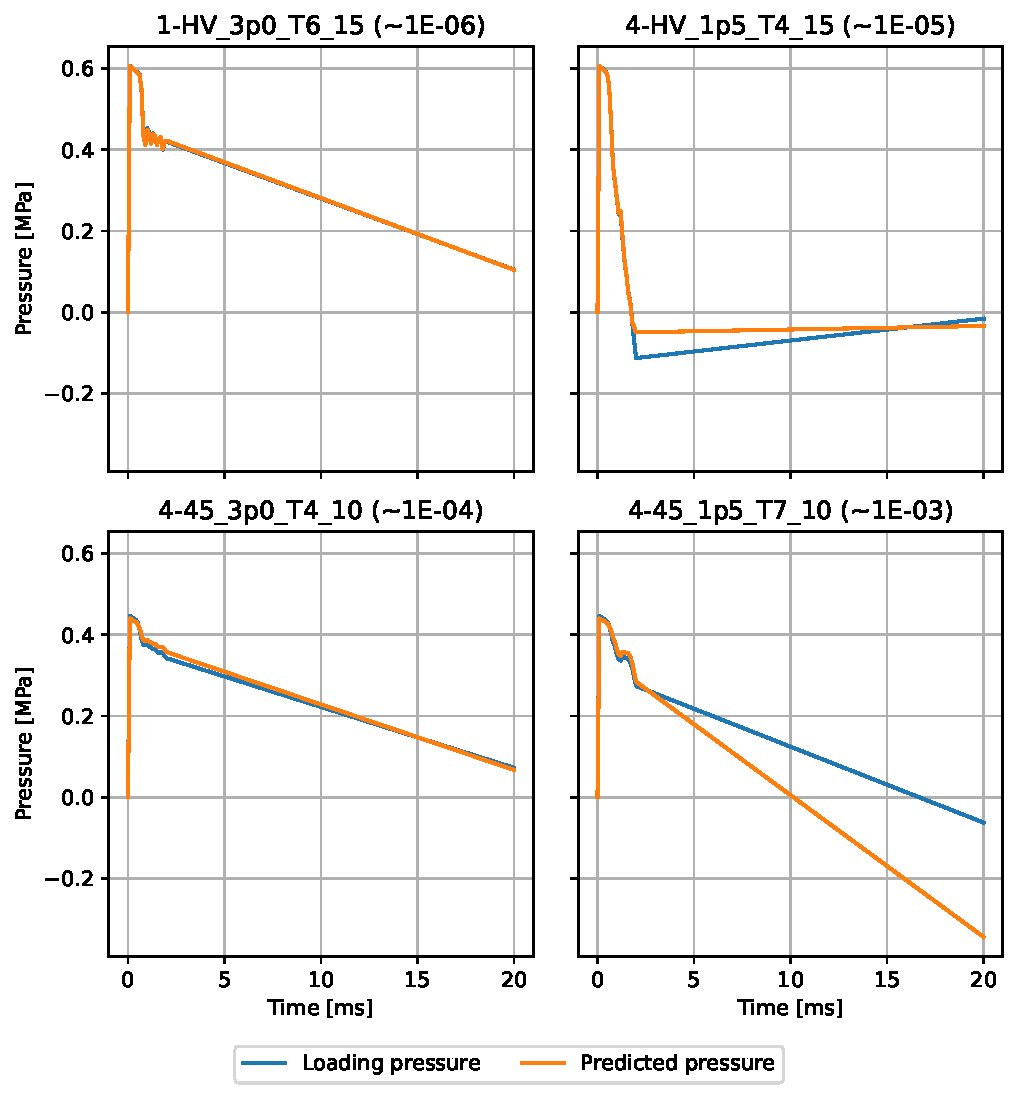
\includegraphics[width=\textwidth]{results/para1_test}
    \caption{Bottom text}
    \label{fig:para1_test}
\end{figure}

\begin{figure}
    \centering
    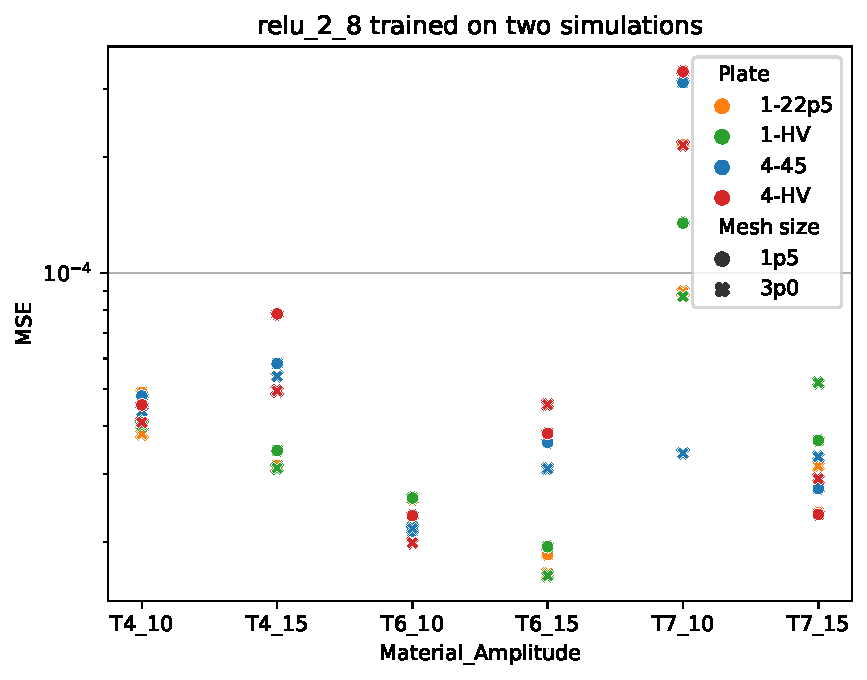
\includegraphics[width=\textwidth]{results/para2_all}
    \caption{Bottom text}
    \label{fig:para2_all}
\end{figure}

\begin{figure}
    \centering
    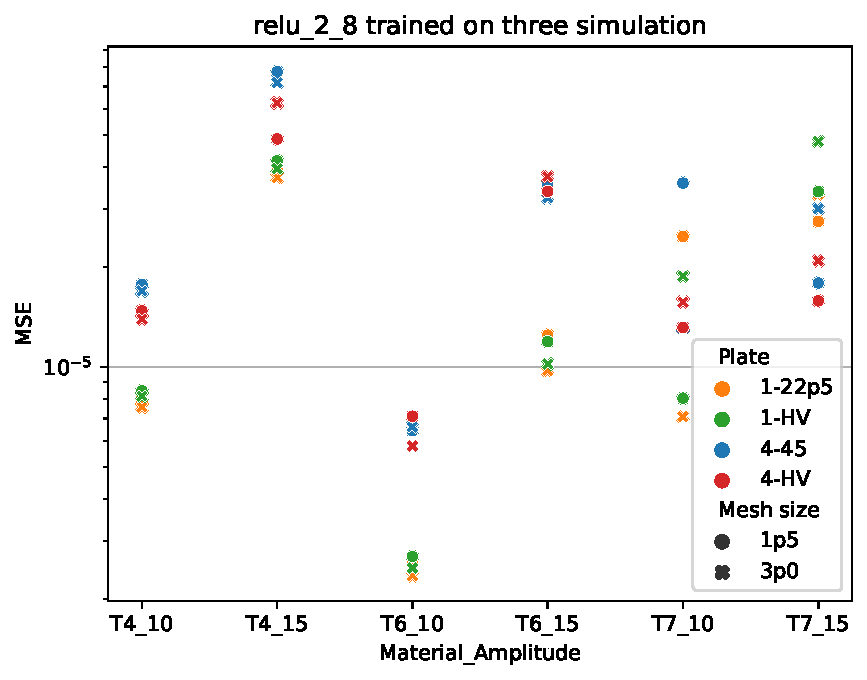
\includegraphics[width=\textwidth]{results/para3_all}
    \caption{Bottom text}
    \label{fig:para3_all}
\end{figure}

\begin{figure}
    \centering
    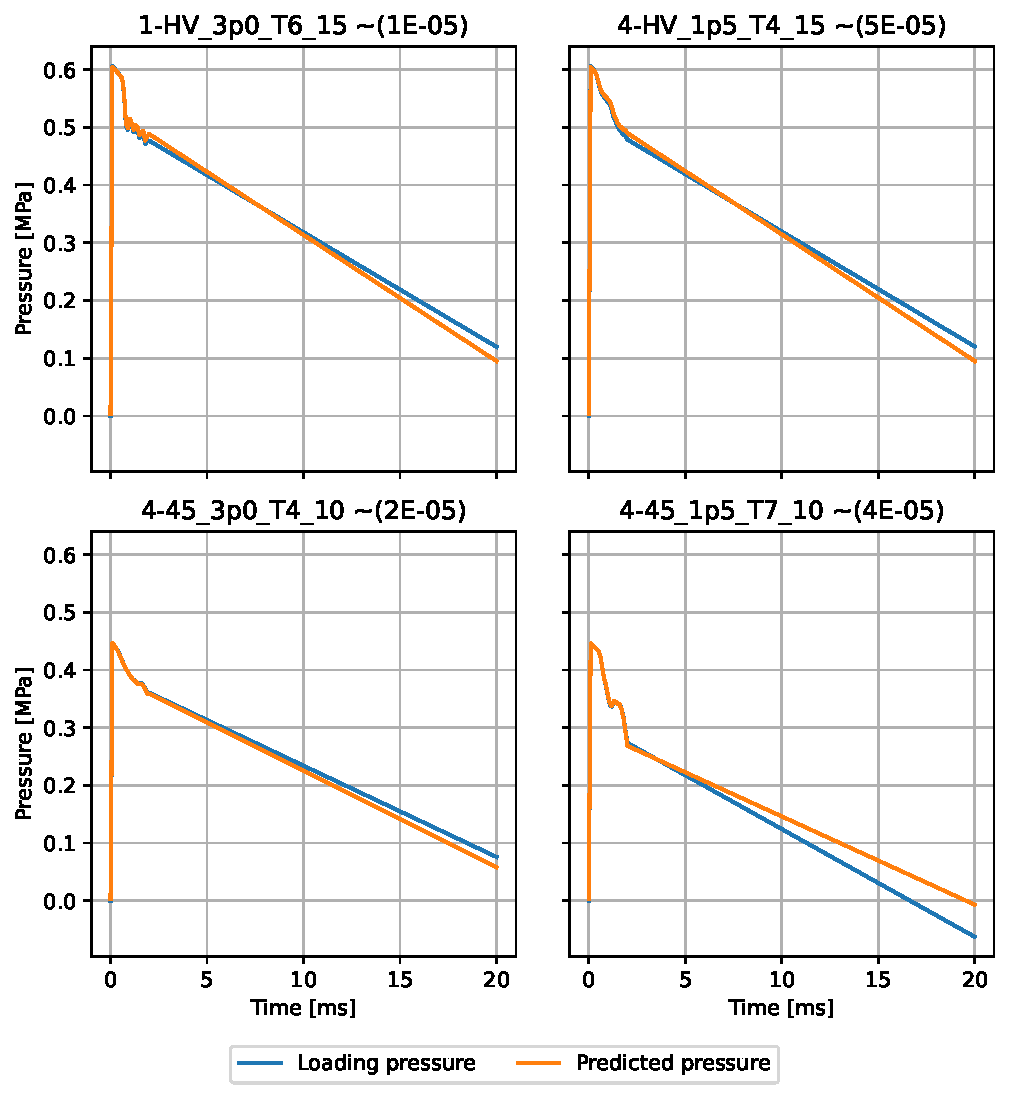
\includegraphics[width=\textwidth]{results/para3_test}
    \caption{Bottom text}
    \label{fig:para3_test}
\end{figure}

\begin{figure}
    \centering
    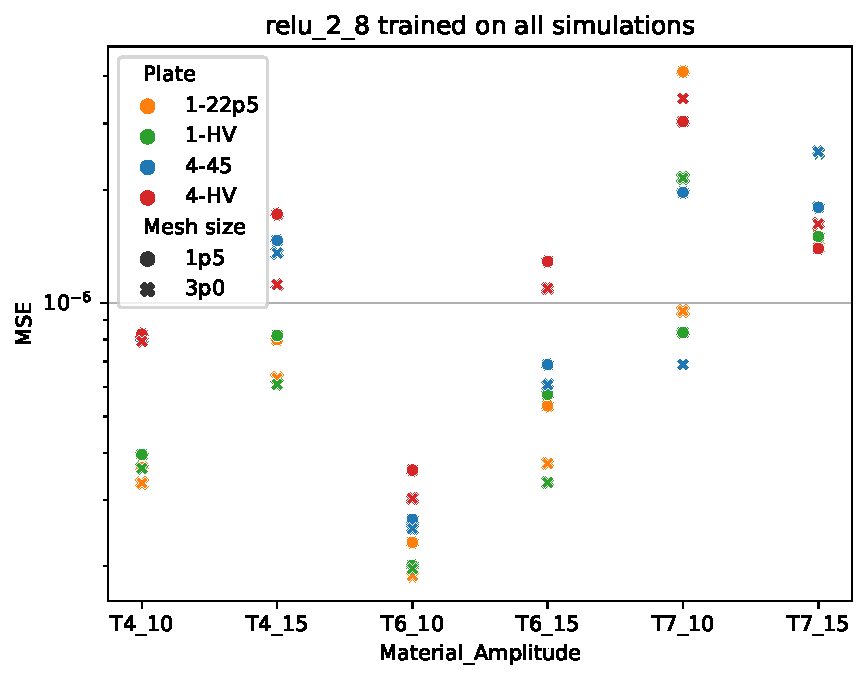
\includegraphics[width=\textwidth]{results/para4_all}
    \caption{Bottom text}
    \label{fig:para4_all}
\end{figure}

\begin{figure}
    \centering
    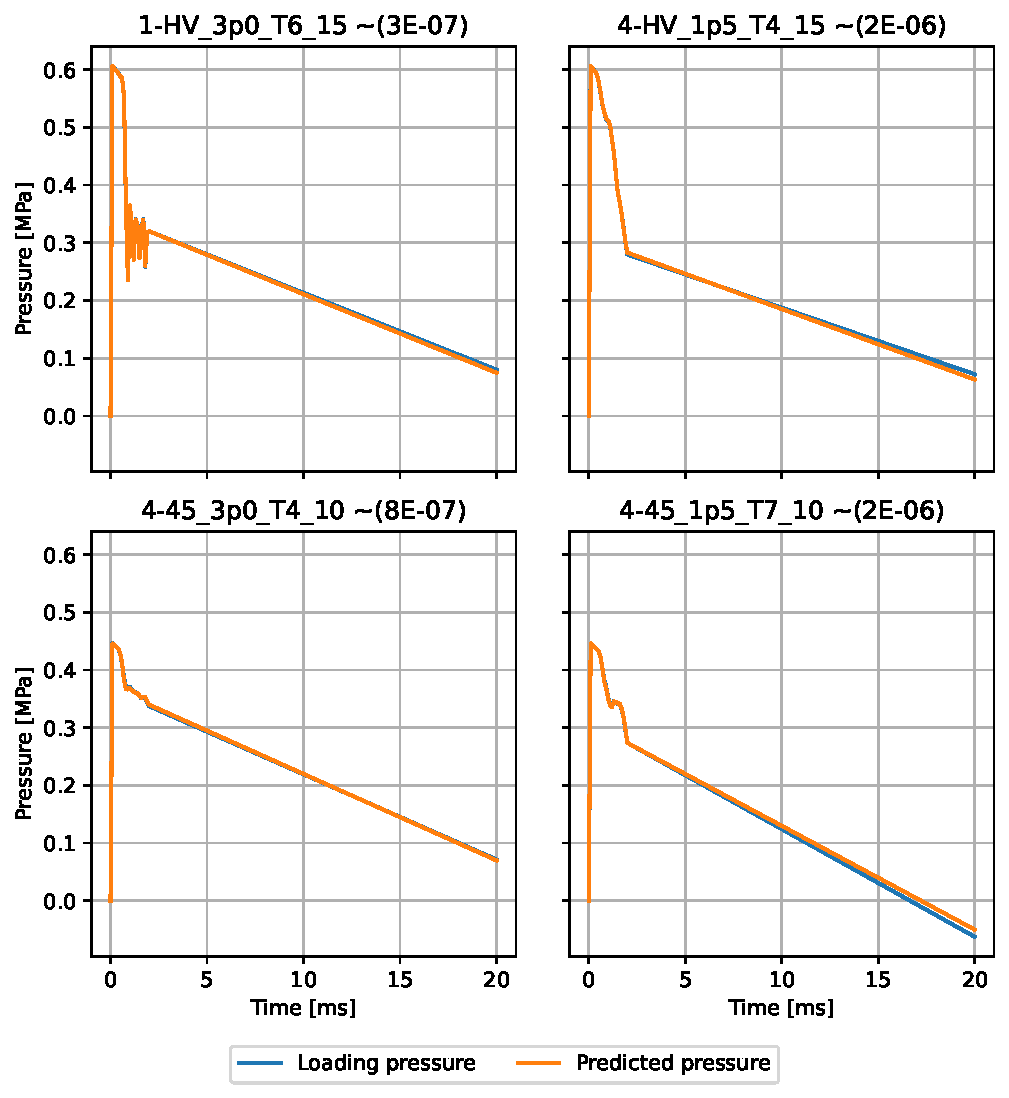
\includegraphics[width=\textwidth]{results/para4_test}
    \caption{Bottom text}
    \label{fig:para4_test}
\end{figure}

\begin{figure}
    \centering
    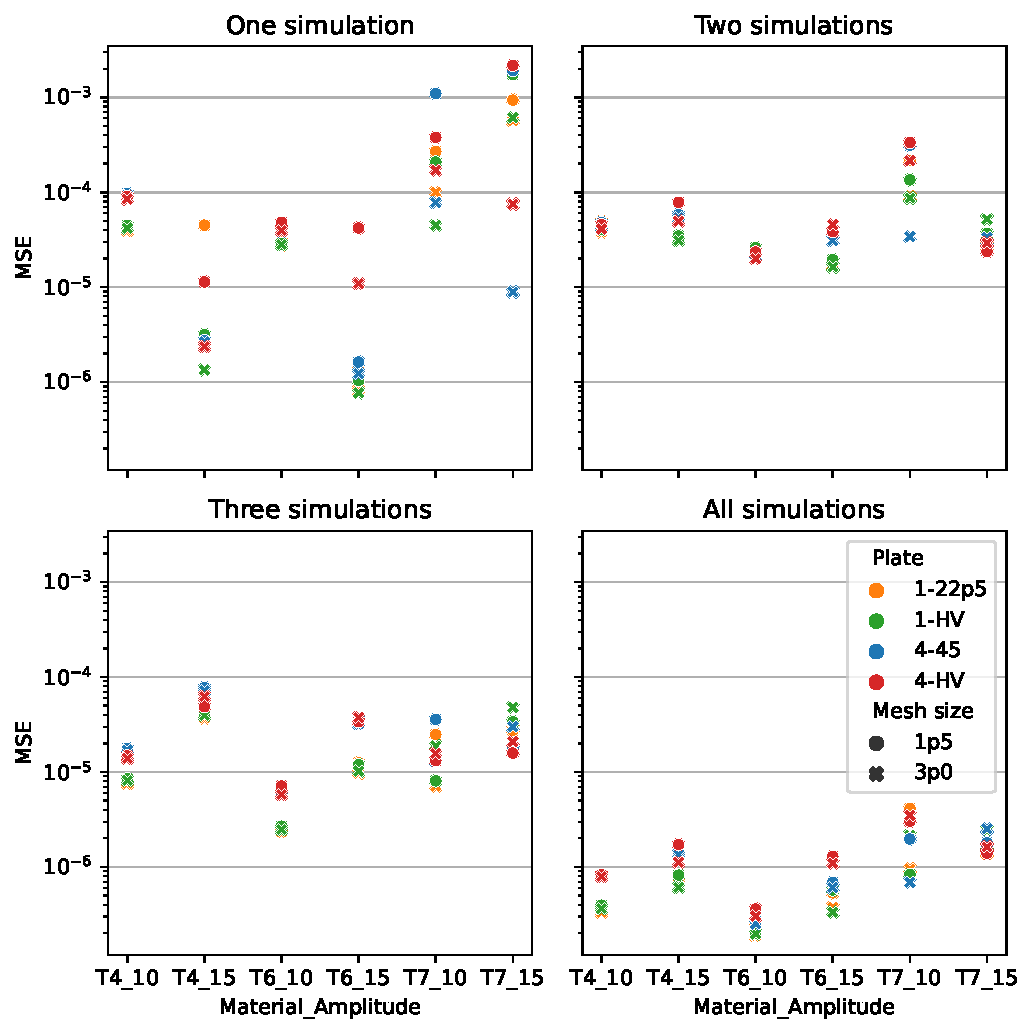
\includegraphics[width=\textwidth]{results/para_all}
    \caption{Bottom text}
    \label{fig:para_all}
\end{figure}

\begin{figure}
    \centering
    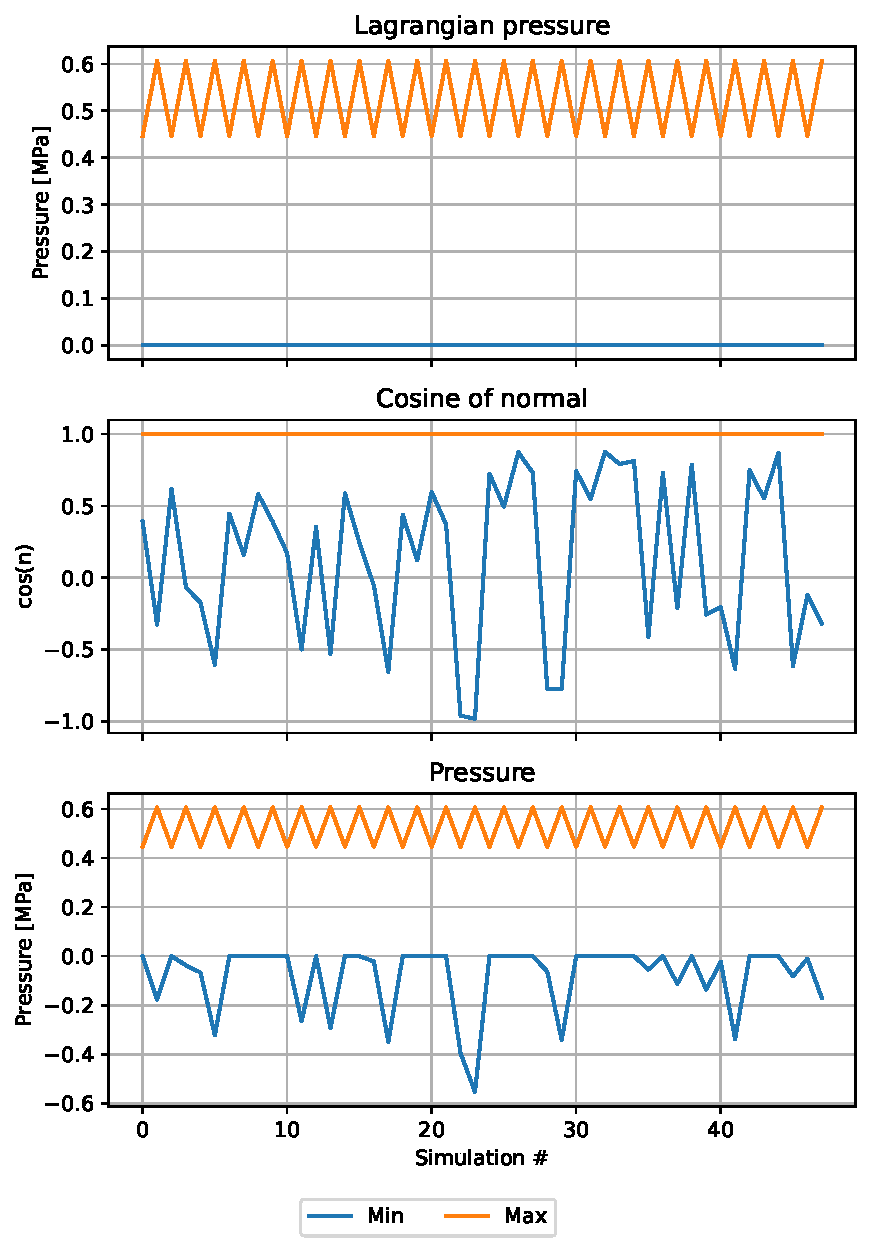
\includegraphics[width=\textwidth]{results/vars}
    \caption{Bottom text}
    \label{fig:para_vars}
\end{figure}

\begin{figure}
    \centering
    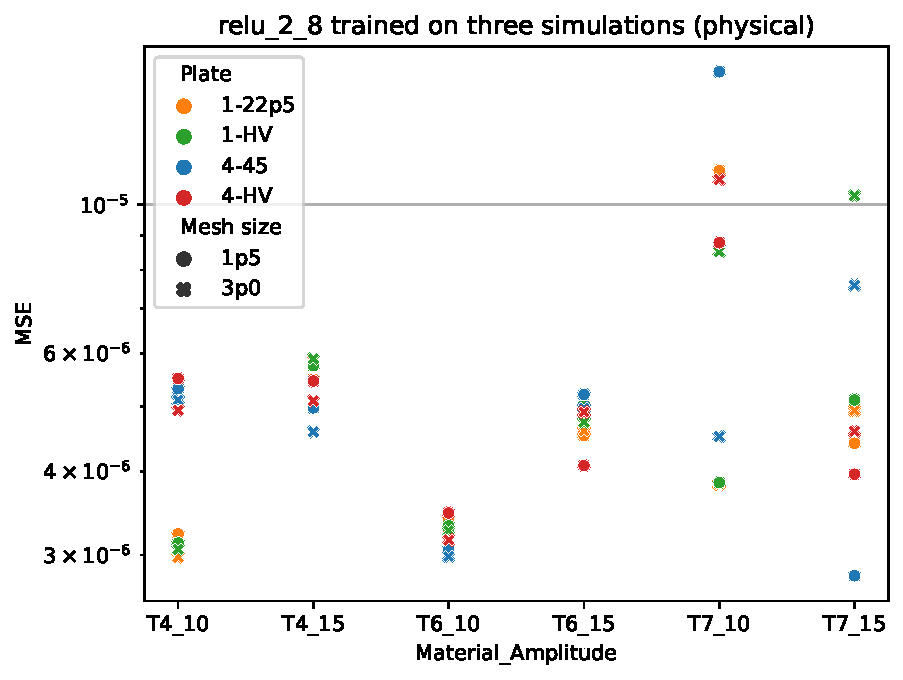
\includegraphics[width=\textwidth]{results/para5_all}
    \caption{Bottom text}
    \label{fig:para5_all}
\end{figure}

\begin{figure}
    \centering
    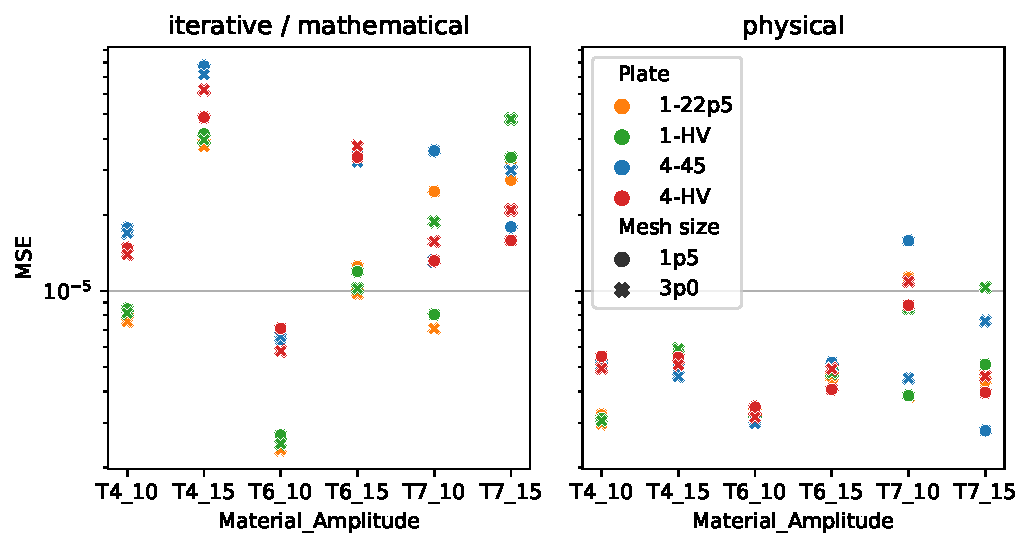
\includegraphics[width=\textwidth]{results/para3_vs_para5}
    \caption{Bottom text}
    \label{fig:para3_vs_para5}
\end{figure}